\chapter{网络功能虚拟化相关技术}
\label{chap:relatedwork}

\section{网络功能虚拟化发展概况}
在2012年10月,“网络功能虚拟化“规范小组在德国达姆施塔特发表了一个关于软件定义网络(SDN)和OpenFlow的白皮书\cite{etsi2012introductory}。该组织是欧洲电信标准协会(ETSI)的一部分,由来自欧洲及其他地区的电信业代表组成。自白皮书发表以来,该小组已经制定了详细的工作计划,更深入的资料,其中包括一个标准的术语定义和用于NFV的使用案例,供供应商和运营商考虑采用网络虚拟化。

\section{常见的网络I/O虚拟化技术}
虚拟化技术提供了在逻辑上划分不同应用程序的系统资源的能力。 I/O虚拟化,特别是网络虚拟化,是实现成功和有效的虚拟化服务器的关键组件。在本节中,我们将介绍和分析三种I/O虚拟化模型:设备仿真,分离驱动程序模型和硬件辅助模型。

\subsection{设备模拟模式}
I / O虚拟化的设备仿真方法通常用于全虚拟化,如图1所示,它通过在虚拟机监视器中虚拟化敏感和特权指令来模拟物理设备的I / O操作
(VMM)层。 这个效果充分利用二进制翻译和直接执行技术的组合来抽象和分离底层硬件形式的客户操作系统。 设备仿真方法为I / O操作提供了最佳性能隔离和安全性,并且简化了迁移和可移植性,因为guest虚拟机操作系统实例和用户级别指令在没有虚拟化意识的情况下不加修改地运行。 使用二进制翻译的设备仿真方法成为事实上的标准VMware产品系列,如VMware Workstation和VMware ESX Server\cite()。 此外,还可以配置XEN和KVM的QEMU来部署I/O虚拟化的设备仿真方法。
\begin{figure}[!htp]
	\centering
	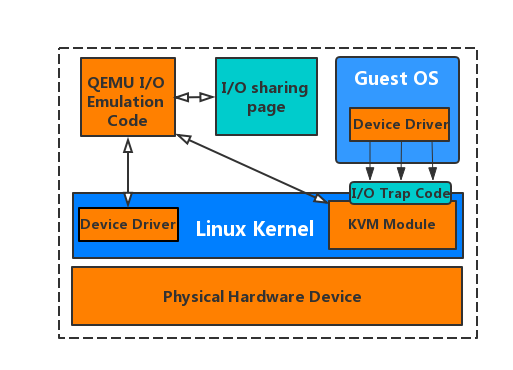
\includegraphics[width=0.8\textwidth]{Device_Emulation.png}
	\bicaption[fig:SRR]{设备模拟模式示意图}{设备模拟模式示意图}{Fig}{Device Emulation Model}
\end{figure}
但是,由于VMM需要动态翻译所有操作系统指令并缓存所有结果,所以设备仿真方法引发了弱故障隔离,因此VMM设备驱动程序的故障将导致所有guest虚拟机的I / O中断。 而且,由于在运行时对这些敏感和特权的指令请求进行代价高昂的陷阱和仿真,所以会导致性能方面的挑战。 据报道,每个典型的I / O操作陷阱和仿真都将导致客户操作系统和VMM之间的上下文切换,其成本约为3000〜5000个CPU周期[13]。 在实践中,它显着降低了我们实验的近10倍的I / O吞吐量。 这一挑战阻碍了将设备仿真方法部署到云计算中的高性能网络和配备现代NIC(例如40 Gbps NIC)的数据中心。

\subsection{Split-driver模式}
为了缓解VMM干预的高开销,PV的分割驱动模型首先由Xen组开发[10],[14]。 KVM的virtio [15],[16],VMware工具和虚拟机接口[17]也可以支持PV的分离驱动模型。 KVM PV的分离驱动模型如图2所示,它由主机中的前端virtio驱动和后端驱动组成。 当虚拟机向服务器内的另一台虚拟机发送数据时,虚拟机首先将数据加载到其Vring缓冲区中的队列,并修改描述符表。然后通知KVM产生vm-exit,并使用ioeventfd允许vHost驱动程序接收来自VM(来宾OS)的信号。
\begin{figure}[!htp]
	\centering
	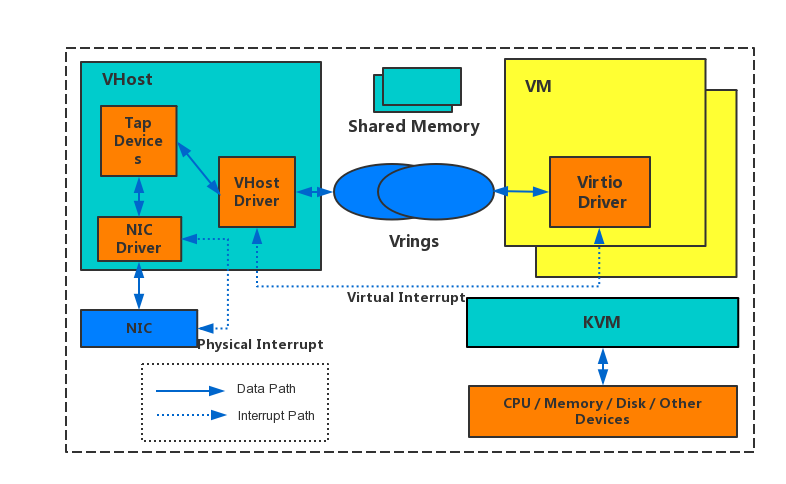
\includegraphics[width=0.8\textwidth]{Split_driver.png}
	\bicaption[fig:SRR]{Split-driver模式示意图}{Split-driver模式示意图}{Fig}{Split-driver Model}
\end{figure}
一旦vHost获得信号,它将获取有效队列的物理地址,并将数据复制到绑定点击设备。数据将通过网络堆栈传输到目的地。如果发现目标是同一台机器上的虚拟机,vHost将利用零拷贝机制,通过共享内存直接将数据复制到目标虚拟机的虚拟环境中。当收到数据时,回调信号将被触发,并让VM将传输的数据放入使用队列。总而言之,虚拟化中的数据流可以被看作是将数据从一个存储区复制到另一个存储区。拆分驱动程序模型采用高效的I / O通信通道(I / O通道),以减少模拟端口I / O和内存映射I / O功能的管理程序干预。因此,拆分驱动程序可以利用主机设备功能提供比设备仿真方法更多的吞吐量和更少的CPU利用率。即使PV需要对操作系统内核进行深度修改,拆分驱动程序模型也显示出其在监督和迁移方面的巨大灵活性,在现代管理程序和来宾域中得到支持


\subsection{硬件辅助模式}
设备仿真和拆分驱动程序模型都被分类为基于软件的I / O虚拟化,从而实现了丰富的功能,简化了管理。 然而,他们遭受的形式是过度的陷阱 - 仿真或大量的数据移动[18]。 因此,硬件辅助I / O虚拟化模型是为本地共享设备而开发的,它通过I / O内存管理单元(IOMMU)的用户继承了直接I / O技术,以卸载内存保护和地址转换。 PCI-SIG给出了规范,通过为每个虚拟机提供独立的内存空间,中断和DMA流来规范绕过VMM参与数据移动的方式。通常情况下,PCI-SIG创建了单根I / O虚拟化(SR-IOV)[19],该设计为PCIe设备设计了一组硬件增强功能,用于移除数据移动的主要VMM干预,如数据包分类和地址转换。
\begin{figure}[!htp]
	\centering
	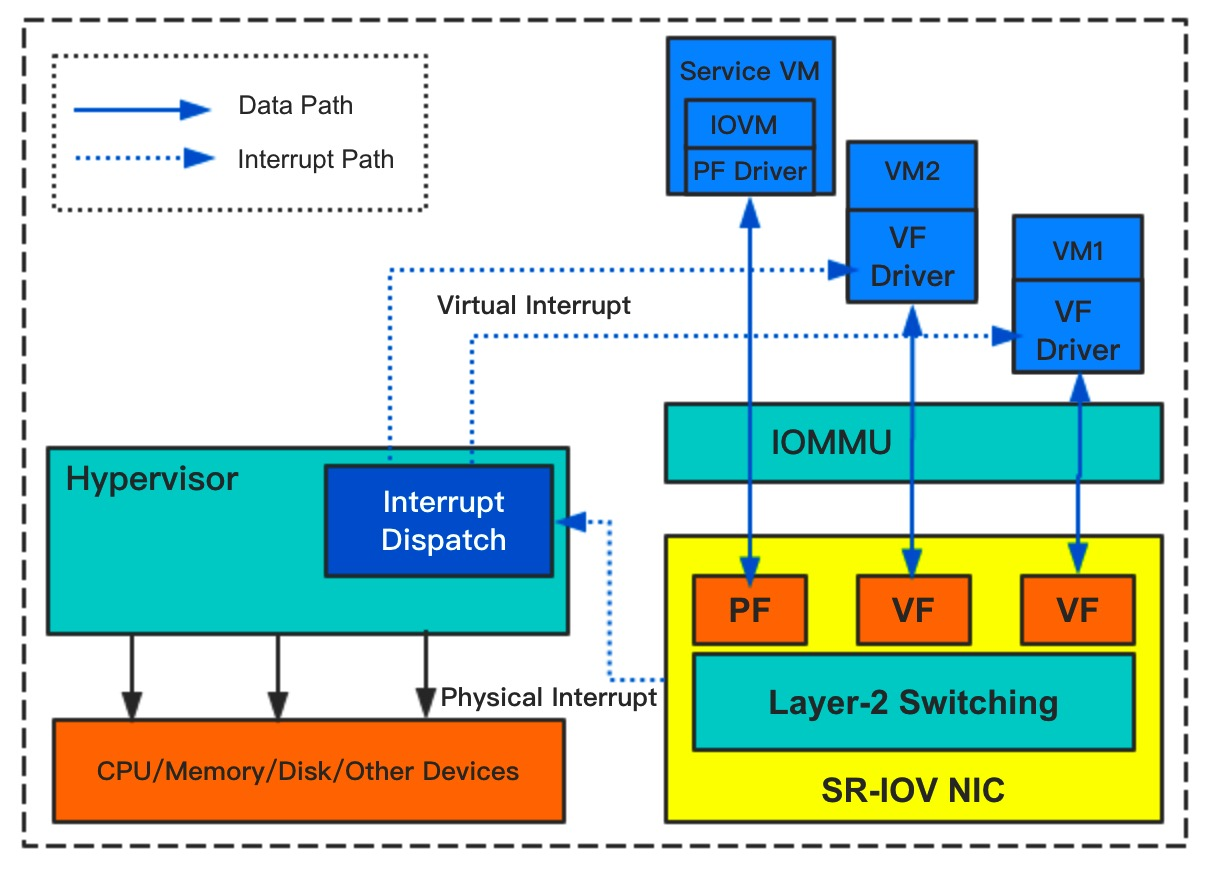
\includegraphics[width=0.8\textwidth]{SR_IOV.jpg}
	\bicaption[fig:SRR]{硬件辅助模式示意图}{硬件辅助模式示意图}{Fig}{Hardware-assisted Model}
\end{figure}
SR-IOV虚拟化体系结构如图3所示,其中一个具有SR-IOV功能的设备可以由VMM配置成在多个虚拟功能(VF)中出现在PCI配置空间中。 具有SR-IOV功能的器件提供可配置数量的独立VF,每个VF具有用基地址寄存器(BAR)完成的自己的配置空间。 服务OS(主机OS)中的物理功能(PF)驱动程序负责管理和配置VF,每个VF驱动程序作为正常的设备驱动程序运行在客户OS上,通过IOMMU直接访问其专用的VF。 因此,SR-IOV可以绕过虚拟机管理程序,以减轻数据移动开销,降低CPU利用率,减少系统延迟并提高网络吞吐量。


\section{非一致性存储访问架构(NUMA)}


\section{本章小结}